\begin{frame}
\frametitle{Renderizzare Un Colore: Demo}
\begin{figure}[ht]
    \centering
    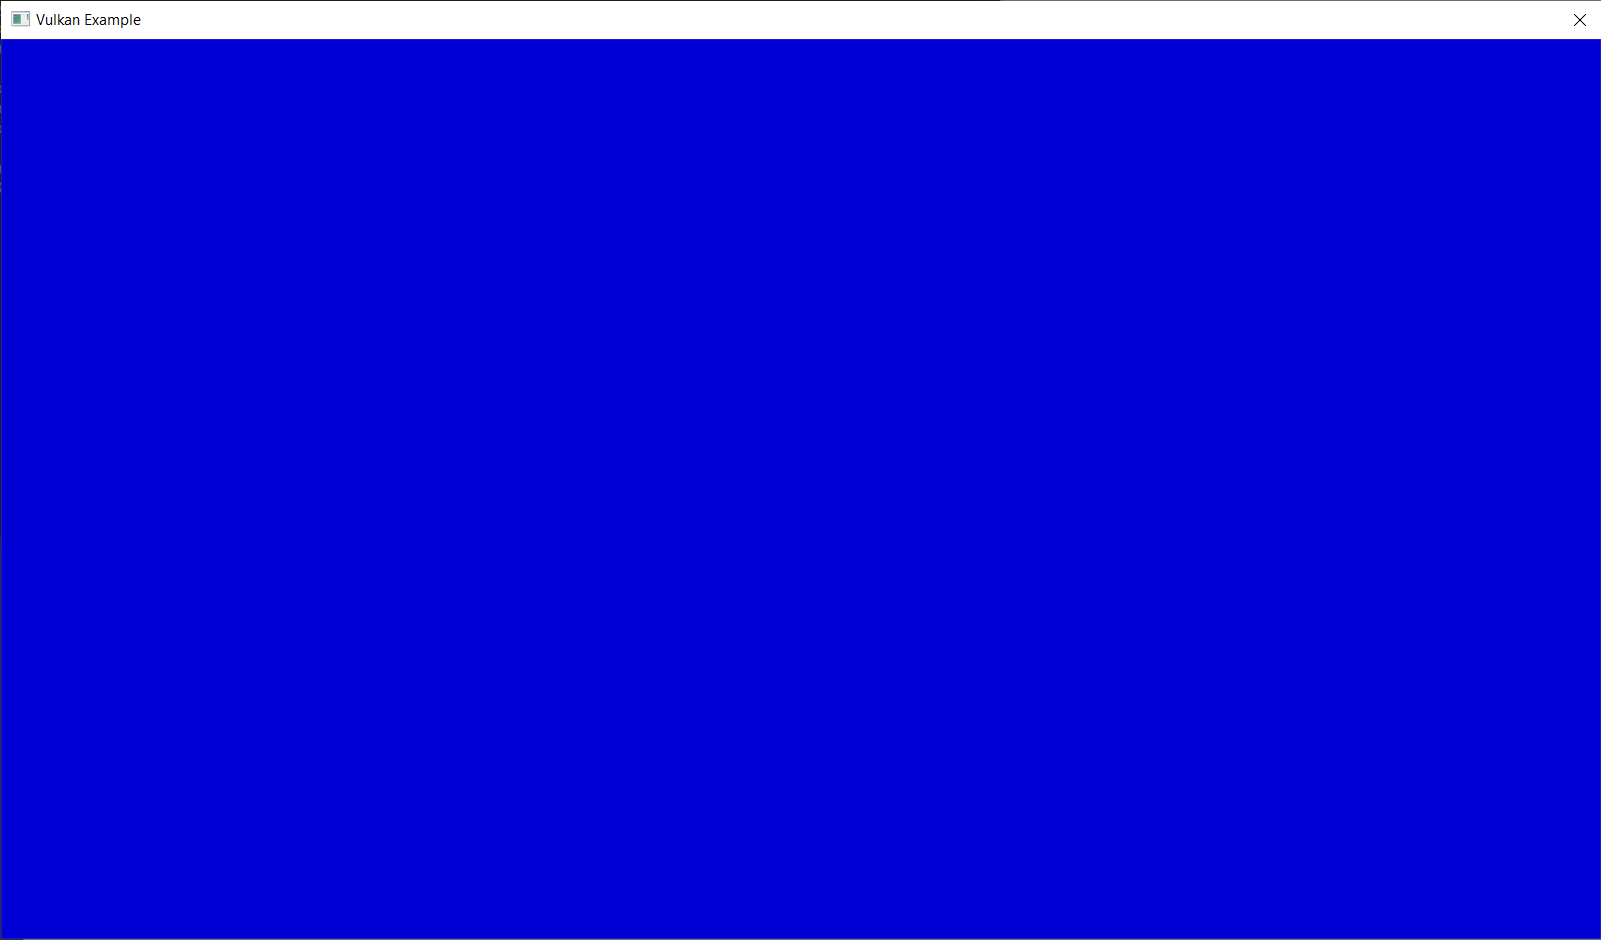
\includegraphics[scale=0.25]{images/SlidesClearWindow/ClearWindow.png}
\end{figure}
\end{frame}

\begin{frame}
\frametitle{Renderizzare Un Colore: Setup}

\begin{itemize}
    \item Creare un command buffer su cui scrivere i comandi grafici da eseguire
    \item Creare un render pass
    \item Un render pass descrive gli attachment che vengono utilizzati durante il rendering
    \item Un render pass raggruppa i comandi grafici in uno o più subpass in base a come e quali attachment questi utilizzano
\end{itemize}
\end{frame}

\begin{frame}
\frametitle{Renderizzare Un Colore: Main Loop}

\begin{itemize}
    \item Ottenere la prossima immagine della swapchain sulla quale renderizzare
    \item Aspettare che i comandi registrati nel command buffer abbiano terminato l'esecuzione
    \item Creare un framebuffer che contiene l'immagine della swapchain
    \item Un framebuffer raccoglie tutti gli attachment che vengono utilizzati durante un'istanza di un render pass
    \item Scrivere sul command buffer due comandi: uno per iniziare il render pass, un'altro per terminarlo
    \item Quando iniziamo il render pass, specifichiamo il clear color per l'immagine
    \item Inviamo il command buffer alla GPU, cosicché questa esegua i comandi registrati
    \item Inviamo un comando di presentazione alla GPU per presentare l'immagine renderizzata
\end{itemize}

\end{frame}
